\subsection{Interface}

Ein\textbf{ User Interface (UI)} in eingebetteten Systemen ermöglicht eine Interaktion zwischen Benutzer und Gerät.

Das \textbf{Interface} besteht aus \textbf{Encodern}, \textbf{Schiebepotentiometern}, einem \textbf{LCD-Display }und \textbf{Buttons}. Dessen Zusammenspiel ermöglicht dem Benutzer die nötige Kontrolle über den Sampler.


Im folgenden Kapitel wird Ihnen die Funktionalität, Implementierung, Ansteuerung, sowie das Zusammenspiel der Komponenten untereinander nähergebracht: 

\subsubsection{Encoder}
\textbf{Komponente \hyperlink{LF01_Link}{/LF01/}} \\

\textbf{Grundfunktionalität:} \\


Der \textbf{Encoder} dient der Navigation im Benutzer-Menü des Samplers. Er ermöglicht die Auswahl von Samples und das Scrollen durch die Sample-Liste, die auf dem LCD-Display angezeigt wird. Diese Liste zeigt die Namen der Samples an, die zuvor durch die Fader-Einstellungen bestimmt wurden. Der Cursor an der Seite zeigt die Aktuelle Position des Cursors an. Der Sample gilt als ausgewählt wen dessen Name unter der Liste erscheint.\\

\textbf{Umsetzung der Funktionalität:} \\

Die Auswahl von Samples sowie das Inkrementieren und Dekrementieren des Cursors, welcher sich im Struct des Filemanager befindet werden durch Interrupts unterstützt. Wenn der Encoder bewegt oder gedrückt wird, sendet er Signale an die MCU, die Interrupts auslösen.\\

Die Auswertung dieser Signale erfolgt dann in der Callback  \mintinline{c}|HAL_GPIO_EXTI_Callback(uint16_t GPIO_Pin)|. 

\begin{figure}[H]
	\centering
	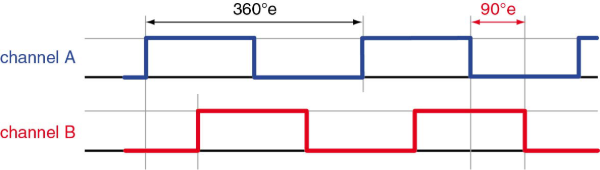
\includegraphics[width=0.8\textwidth]{images/08_durchfuehrung/interface/encoder.png}
	\caption{Phasenverschiebung A und B}
	\label{fig:phase_verschiebung}
\end{figure}

Wenn A und B beide High sind, wird die Cursor-Position welche in auf dem Display durch den Methodenaufruf \mintinline{c}|cursorUp(FileManager *fm)|
erhöht. Wenn  \textbf{\autoref{fig:phase_verschiebung}} A High und B Low ist, wird die Cursor-Position auf dem Display durch \mintinline{c}|cursorDown(FileManager *fm)| verringert. Wenn der Schalter gedrückt wird, wird die Datei durch \mintinline{c}|selectFile(FileManager *fm)| der Index des Files gespeichert. 

\newpage 
 \inputminted[firstline=68, lastline=74]{c}{../../f401_display_encoder_fader_test/Core/Src/filemanager.c}
 
  \inputminted[firstline=84, lastline=90]{c}{../../f401_display_encoder_fader_test/Core/Src/filemanager.c}
  
Anhand des Index des Files kann der Names des Files ermittelt werden.

	
\inputminted[firstline=159, lastline=161]{c}{../../f401_display_encoder_fader_test/Core/Src/filemanager.c}

\textbf{Problematik:}

Beim Drücken des Knopfes kann es in Systemen zu Mehrfachauslösungen kommen. Dies war auch beim Schalter des Encoders der Fall.

\textbf{Lösung:}

Um Mehrfachauslösungen zu verhindern, wurde ein Debouncing-Mechanismus implementiert. Dieser Mechanismus verwendet ein Flag \mintinline{c}|debounce| und einen Timer \mintinline{c}|tim3|, um wiederholte Auslösungen zu verhindern. Beim Drücken des Knopfes wird ein Interrupt ausgelöst, der eine Callback-Funktion \mintinline{c}|HAL_GPIO_EXTI_Callback(uint16_t GPIO_Pin)| aufruft. In dieser Callback-Funktion wird ein Flag gesetzt und ein Timer gestartet. Der Timer sorgt dafür, dass weitere Auslösungen innerhalb einer definierten Zeitspanne ignoriert werden, wodurch Mehrfachauslösungen effektiv verhindert werden.

Erst nach dem Ablauf des Timers war ist ein möglich den Knopf wieder zu betätigen.

\newpage
\subsubsection{Schiebenpotentiometer, ADC und DMA}
\textbf{Komponenten\hyperlink{LF02_Link}{/LF02/}} \\

\textbf{Grundfunktionalität:}\\

\textbf{Schiebepotentiometer} erfassen analoge Spannungen, die vom \textbf{Analog-Digital-Wandler (ADC)} in digitale Werte umgewandelt werden\textbf{\autoref{fig:conversion}}. Er nimmt in regelmäßigen Intervallen Proben des analogen Signals. Die Auflösung in 12 Bits 15 ADC Clock Cycles hat sich als am effizientesten herrausgestelt. ()\textbf{Wertebereich} 0-4096).

\begin{figure}[H]
	\centering
	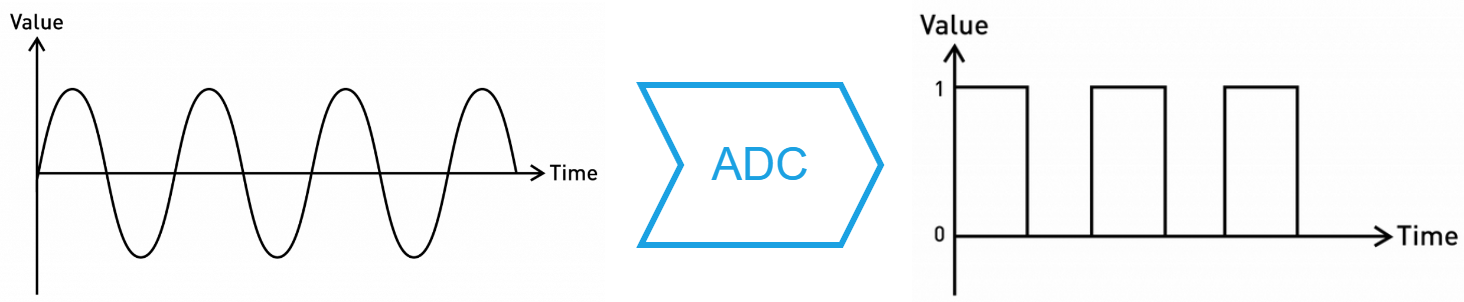
\includegraphics[width=1.0\textwidth]{images/08_durchfuehrung/interface/Conversion.drawio.png}
	\caption{ADC Conversion}
	\label{fig:conversion}
\end{figure}

Der \textbf{Direct Memory Access (DMA)-Controller} übernimmt anschließend die direkte Übertragung dieser digitalen Werte in den Speicher, konkret in  \mintinline{c}|adcBuffer[NUM_CHANNELS]|.

\begin{figure}[H]
\centering
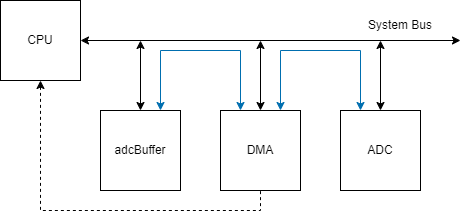
\includegraphics[width=0.8\textwidth]{images/08_durchfuehrung/interface/DMA_ADC_MEM.drawio.png}
\caption{DMA ADC FADER Bus System}
\label{fig:DMA_ADC_FADER}
\end{figure}

Der Direct Memory Access (DMA)-Controller ermöglicht die direkte Datenübertragung zwischen Speicher und Peripheriegeräten, wodurch die Prozessorbelastung reduziert wird. Analoge-Digital-Wandler (ADCs) sorgen für die schnelle Digitalisierung analoger Signale, was eine präzise Verarbeitung der Messdaten ermöglicht. Potentiometer bieten die Möglichkeit zur benutzerfreundlichen Anpassung von Spannungswerten. Das Bussystem sorgt für eine effiziente Kommunikation zwischen den verschiedenen Komponenten und gewährleistet eine konsistente und zuverlässige Datenverarbeitung. \textbf{\autoref{fig:DMA_ADC_FADER}} \\

\newpage
\textbf{Problematik:}

\textbf{No.1}

Bei der Implementierung der DMA traten Probleme auf, die dazu führten, dass der Bildschirm einfrohr und das Bedienen der Interfaces unmöglich wurde. Das Problem entstand, weil die DMA fortlaufend Daten übertrug und die CPU dadurch vollständig beansprucht wurde, um die Daten, die von der DMA übertragen wurden, zu verarbeiten. Dies führte zu einer Überlastung der CPU, da sie gezwungen war, sich auf die Verarbeitung der von der DMA bereitgestellten Daten zu konzentrieren, anstatt andere Aufgaben zu bewältigen. Infolgedessen konnten keine weiteren Systeminteraktionen durchgeführt werden, da die CPU keine Ressourcen mehr für andere Aufgaben zur Verfügung hatte.

\textbf{No.2}

Die Auswertung und Verarbeitung der Signale erfolgt in der \mintinline{c}| HAL_ADC_ConvCpltCallback(ADC_HandleTypeDef* hadc)|.

Im laufe der Implementation des ADC könnte man Schwankungen an den Ausgangssignalen des ADCs festellen, was die Genaugigkeit der Potentiometer einstellung beeinflüsste. 

\textbf{Lösung No.1:}

Um das Problem zu beheben, wurde ein \textbf{Timer} \mintinline{c}|tim5| implementiert, der die DMA-Übertragung steuert. Der Timer sorgt dafür, dass die DMA in regelmäßigen Intervallen gestartet und gestoppt wird. Diese Maßnahme ermöglicht es der CPU, sich ausreichend um andere Aufgaben zu kümmern, indem sie nicht kontinuierlich mit der Datenverarbeitung durch die DMA beschäftigt ist. Der Einsatz des Timers verhindert, dass die DMA die CPU überlastet und gewährleistet eine ausgewogene Nutzung der Systemressourcen. \\

\textbf{Lösung No.2:}

Diese Schwankungen würden behoben in dem man ein Glättung der Werte eingeführt hat.

Zunächst werden des \mintinline{c}|adcBuffer[i]| in \mintinline{c}|smoothValue[i]| aufeinander addiert. Dann wird derren Durchschnittswerte berechnet. Die geglätteten Werte werden für alle Kanäle des ADC berechnet. 

\textcolor{red}{TODO: Code Verschieben}

 \inputminted[firstline=121, lastline=135]{c}{../../f401_display_encoder_fader_test/Core/Src/interface.c}

Diese Glättung sorgt dafür, dass die Messwerte stabiler und weniger anfällig für zufällige Schwankungen sind. Anschließend werden die Durchschnittswerte ermittelt. Diese Durchschnittswerte dienen zwei Zwecken: Einerseits werden sie zur Anzeige auf dem Bildschirm verwendet  \mintinline{c}|currentClassPercentADC[]|
, andererseits sind sie für Vergleichsoperationen innerhalb des Sortieralgorithmus von Bedeutung  \mintinline{c}|fm.fader_Class[]|.
 Schließlich wird ein Zeichenarray \mintinline{c}|faderProzent[0]| initialisiert, das später auf dem Display angezeigt wird. 
 
Eine andere möglichkeit des Spannungs inkonsitenz könnte mit Kondensatoren umgesetzt werden was jedoch nicht umgesetzt würde aus zeitlichen Gründen.

\newpage
\subsubsection{Display, SD1306 Treiber und I2C}

\textbf{I2C} \\

\textbf{I2C} (Inter-Integrated Circuit) ist ein Kommunikationsprotokoll, das über zwei Leitungen arbeitet: \textbf{SDA} (Serial Data Line) und \textbf{SCL} (Serial Clock Line). Es verwendet eine Master-Slave-Architektur, bei der der Master die Kommunikation steuert und die Slaves Daten empfangen oder senden. Die Datenübertragung erfolgt in Byte-Paketen, wobei der Master eine Start-Bedingung sendet, gefolgt von der Adresse des Slaves und den Daten. Nach dem Empfang eines Datenbytes sendet der Slave ein Bestätigungsbit (ACK). Die Kommunikation endet mit einer Stop-Bedingung \textbf{\autoref{fig:I2C}}. \\

\textbf{Vorteile}\\

\begin{itemize}
	\item \textbf{Einfache Verkabelung}: Es werden nur zwei Leitungen für die Kommunikation benötigt, was den Verkabelungsaufwand erheblich reduziert.
	\item \textbf{Geringe Hardware-Kosten}: Die Implementierung von I2C ist kostengünstig und benötigt wenig zusätzliche Hardware, da die Logik für das Protokoll minimal ist.
	\item \textbf{Fehlererkennung}: \textbf{I2C} bietet einfache Methoden zur Fehlererkennung, wie das Bestätigungsbit (ACK), um sicherzustellen, dass Daten erfolgreich übertragen wurden.
	\item \textbf{Unterstützung von Standard-Bibliotheken}: Viele Mikrocontroller und Entwicklungsplattformen bieten Standard-Bibliotheken für \textbf{I2C}, was die Implementierung und Fehlerbehebung erleichtert.
\end{itemize}

\begin{figure}[H]
	\centering
	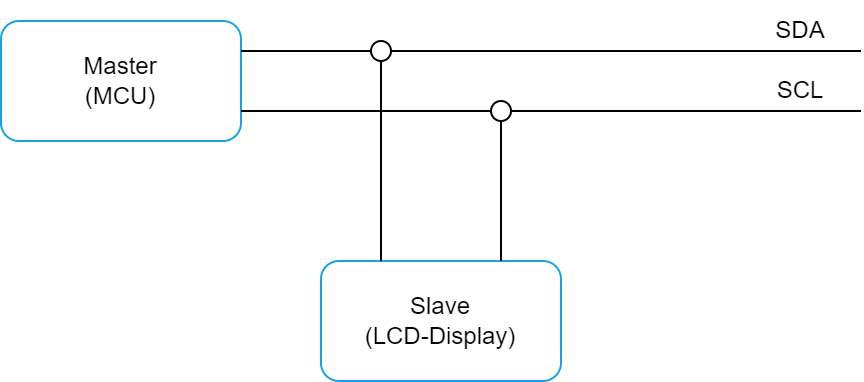
\includegraphics[width=0.8\textwidth]{images/08_durchfuehrung/interface/I2C.drawio.png}
	\caption{I2C Kommunikation}
	\label{fig:I2C}
\end{figure}

\newpage	
\textbf{Display} \\	


Das Display ist die zentrale Komponente des Interfaces, da es visuelles Feedback auf die Benutzerinteraktionen bietet. Die Kommunikation zwischen dem Nucleo F401RE-Mikrocontroller und dem Display erfolgt über das I2C-Protokoll. Der Mikrocontroller übernimmt dabei die Rolle des Masters, der den Bus steuert, während das Display als Slave agiert.

Die Ansteuerung des Displays erfolgt über den SD1306-Treiber, der als Schnittstelle zwischen dem Mikrocontroller Nucleo F401RE und dem LCD-Display fungiert. Der Treiber nutzt das I2C-Protokoll, um Befehle und Daten effizient zu übermitteln. Er sendet die erforderlichen Befehle an das Display und übernimmt die Kommunikation gemäß den I2C-Spezifikationen. Bei Bedarf kann die Initialisierungssequenz des Treibers angepasst werden, um auch SH1103-kompatible Bildschirme zu unterstützen \textbf{\autoref{fig:Display SD1306 I2C}}.

Zusammenfassend ermöglicht der SD1306-Treiber die vollständige Integration des Displays in das System, indem er die I2C-Kommunikation zwischen Mikrocontroller und Display umsetzt. \\ 


\begin{figure}[H]
	\centering
	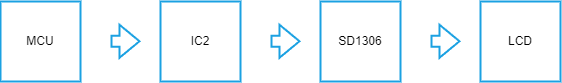
\includegraphics[width=1.0\textwidth]{images/08_durchfuehrung/interface/Display SD1306 Treiber I2C.drawio}
	\caption{Display SD1306 I2C Kommunikation}
	\label{fig:Display SD1306 I2C}
\end{figure}

Die beiden Hauptfunktionen zur Darstellung auf dem OLED-Bildschirm sind:

 \mintinline{c}|void  displayStrings(I2C_HandleTypeDef *hi2c1, char** strings, uint8_t numStrings, uint8_t cursor_index)|
 
 \mintinline{c}|void renderSelectedFile(I2C_HandleTypeDef *hi2c1, const char *filename)| bzw. 
 
 \mintinline{c}|drawFaderProzent| ähnliche funktionsweiße wie  \mintinline{c}|renderSelectedFile|. 


In der Funktion \mintinline{c}|displayStrings| werden die `ssd1306`-Funktionen verwendet, um die Strings auf dem LCD-Display darzustellen. Die Funktion \mintinline{c}|ssd1306_SetCursor| legt die Position für die Anzeige fest, und \mintinline{c}|ssd1306_WriteString| wird verwendet, um die Strings auf dem Display auszugeben. Bei der Anzeige des ausgewählten Strings wird zusätzlich ein Cursor-Symbol integriert.

In der Funktion \mintinline{c}|renderSelectedFile| wie bei \mintinline{c}|displayStrings| `ssd1306`-Funktionen verwendet, um den Namen der ausgewählten Datei auf dem OLED-Display darzustellen. Die Funktion \mintinline{c}|ssd1306_DrawPixel| wird verwendet, um den Bereich für die Dateianzeige zu löschen. Anschließend legt \mintinline{c}|ssd1306_SetCursor| die Position für die Textausgabe fest, und \mintinline{c}|ssd1306_WriteString| gibt den Namen der ausgewählten Datei auf dem Display aus. \\

\textbf{Problematik:} \\

Der ursprünglich verwendete SD1306-Treiber war nicht mit dem Display kompatibel. Der Fehler wurde durch die ungeeignete Initialisierungssequenz für das Display verursacht, was zu einer fehlerhaften Darstellung der Daten auf dem Bildschirm führte.

\textbf{Lösung:} \\

Die Anpassung der Definitionskonstanten, die als Befehle über I2C an das Display gesendet werden, sowie die Änderung der Schleifenbedingung in der Methode \mintinline{c}|ssd1306_UpdateScreen(I2C_HandleTypeDef *hi2c)| von einer Länge von 8 auf 16 haben das Problem behoben.
\newpage


\subsubsection{Dateisystem} 
\vspace{1em}

Das Dateisystem fungiert als zentrale Schnittstelle zwischen der Audio-Wiedergabe, dem neuronalen Netzwerk zur Klassifizierung und der Benutzeroberfläche. Es organisiert und verwaltet die Audiodateien, die vom neuronalen Netzwerk analysiert und klassifiziert werden. Nach der Klassifizierung speichert das Dateisystem die Ergebnisse und gewährleistet, dass nur relevante und korrekt kategorisierte Dateien im Interface angezeigt werden. Das Dateisystem besteht aus zwei Hauptstrukturen: File und FileManager welche Ihnen im folgenden nähr gebracht werden.

\vspace{1em}
\textbf{File}
\vspace{1em}

Die \boldinline{File}-Struktur repräsentiert einzelne Audiodateien im System. Sie enthält den Dateinamen, der sowohl für das Abspielen der Audiodatei als auch für die Anzeige in einer Liste von Samples verwendet wird. Zusätzlich speichert die Struktur Klassifizierungsdaten, die vom neuronalen Netzwerk bereitgestellt werden.


 \inputminted[firstline=37, lastline=41]{c}{../../f401_display_encoder_fader_test/Core/Inc/filemanager.h}
 
\vspace{1em}
\textbf{FileManager}
\vspace{1em}

Die \boldinline{FileManager}-Struktur repräsentiert das Dateisystem selbst. Sie ist verantwortlich für die Verwaltung und Speicherung von Dateien und umfasst wesentliche Elemente, die für die Visualisierung der Dateien auf dem LCD-Display erforderlich sind.
 
 \inputminted[firstline=49, lastline=58]{c}{../../f401_display_encoder_fader_test/Core/Inc/filemanager.h}
 
\vspace{1em} 
\textbf{Problematik:} \\



Das Schreiben der \boldinline{FileManager}-Struktur auf die SD-Karte war zunächst nicht möglich und konnte aus zeitlichen Gründen nicht behoben werden.



